%
% Learning when to grasp
% Invited paper at CLEA/ICRA 2007
% Castellini, Sandini
%

\documentclass[a4paper,10pt,conference]{ieeeconf}

\IEEEoverridecommandlockouts
\overrideIEEEmargins

\usepackage{float}
\usepackage{graphicx}
\usepackage{url}
\usepackage{amsmath}
\usepackage[psamsfonts]{amssymb}

\def\RR{\mathbb{R}}
\def\NN{\mathbb{N}}
\def\xx{\mathbf{x}}
\def\yy{\mathbf{y}}
\def\ww{\mathbf{w}}
\def\aa{\boldsymbol{\alpha}}
\def\bb{\boldsymbol{\beta}}
\def\ee{\mathbf{e}}
\def\dd{\mathbf{d}}
\def\mdd{\tilde{\dd}}
\def\b{\mathcal{B}}
\def\d{\mathcal{D}}

%%%%%%%%%%%%%%%%%%%%%%%%%%%%%%%%%%%%%%%%%%%%%%%%%%%%%%%%%%%%%%%%%%%%%%%%%%%%%%%%
\title{\LARGE \bf Learning when to grasp}

\author{Claudio Castellini and Giulio Sandini%
\thanks{Claudio Castellini (corresponding author) is
with the LIRA-Lab, University of Genova,
viale F. Causa 13, 16145 Genova, Italy. Email
{\tt\small claudio.castellini@unige.it}}%
\thanks{Giulio Sandini is with the Italian Institute of Technology,
via Morego 16, 16100 Genova, Italy. Email
{\tt\small giulio.sandini@iit.it}}%
}

\begin{document}

\maketitle
\thispagestyle{empty}
\pagestyle{empty}

%%%%%%%%%%%%%%%%%%%%%%%%%%%%%%%%%%%%%%%%%%%%%%%%%%%%%%%%%%%%%%%%%%%%%%%%%%%%%%%%
\begin{abstract}

In critical human/robotic interactions such as, e.g., teleoperation by
a disabled master or with insufficient bandwidth, or intelligent
prostheses, it is highly desirable to have \emph{semi-autonomous}
robotic artifacts interact with a human being. Semi-autonomous
teleoperation, for instance, consists in having a smart slave able to
guess the master's intentions and possibly take over control in order
to perform the desired actions in a more skillful/timely way than with
plain, point-to-point teleoperation.

In this paper we investigate the possibility of building such an
intelligent robotic artifact by training a machine learning system on
data gathered from several human subjects while trying to grasp objects
in a teleoperation setup. The idea is to have the slave ``guess'' when
the master wants to grasp an object with the maximum possible
accuracy; at the same time, the system must be light enough to be
usable in an on-line scenario and flexible enough to adapt to
different masters, e.g., elderly and/or slow.

The outcome of the experiment is that such a system, based upon
Support Vector Machines, meets all the requirements, being $(a)$
highly accurate, $(b)$ compact and fast, and $(c)$ largely unaffected
by the subjects' diversity. The system is, moreover, trained by
something like $3.5$ minutes of human data in the worst case.

\end{abstract}

%%%%%%%%%%%%%%%%%%%%%%%%%%%%%%%%%%%%%%%%%%%%%%%%%%%%%%%%%%%%%%%%%%%%%%%%%%%%%%%%
\section{INTRODUCTION}

\begin{figure*}[ht]
  \centering
    \begin{tabular}{ccc}
      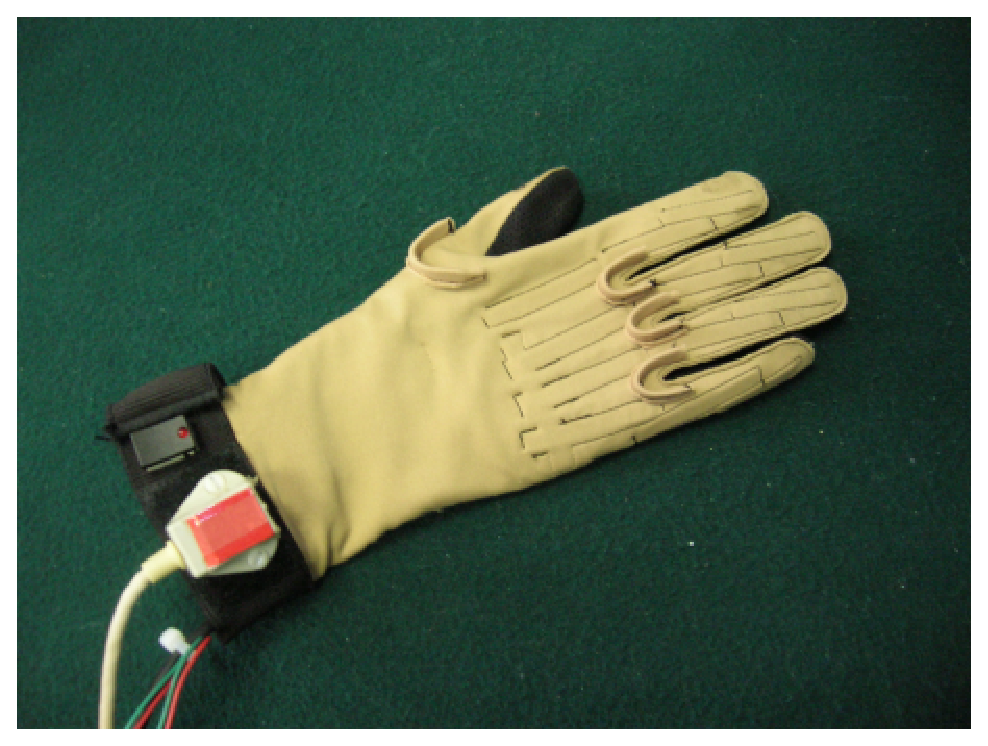
\includegraphics[width=0.31\linewidth]{glove.eps} &
      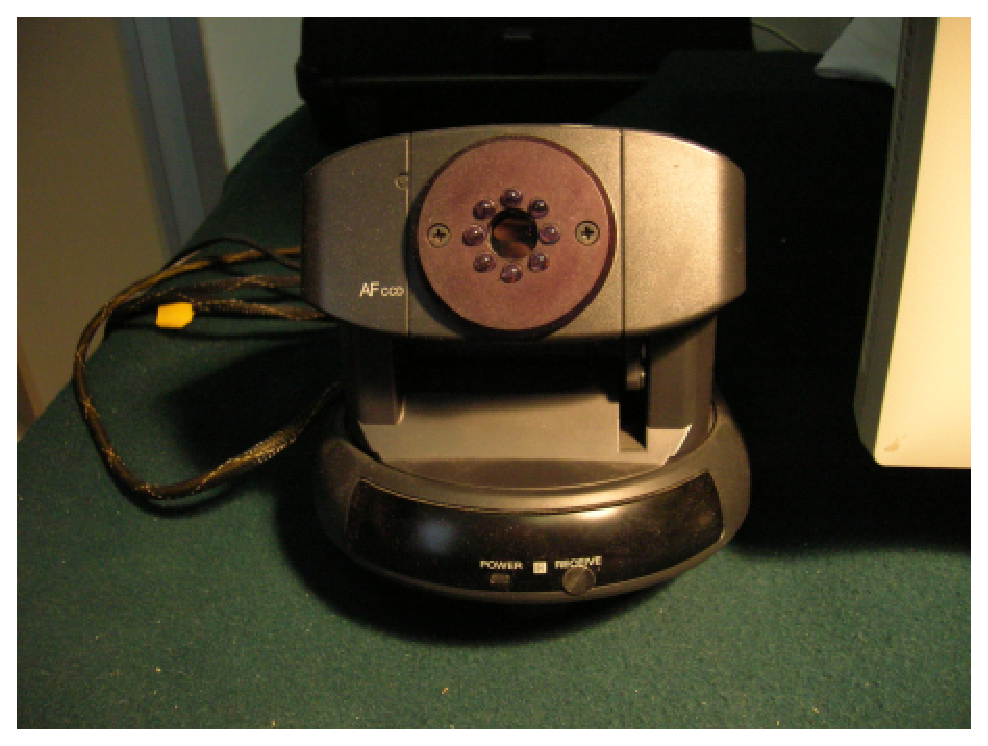
\includegraphics[width=0.31\linewidth]{e504.eps} &
      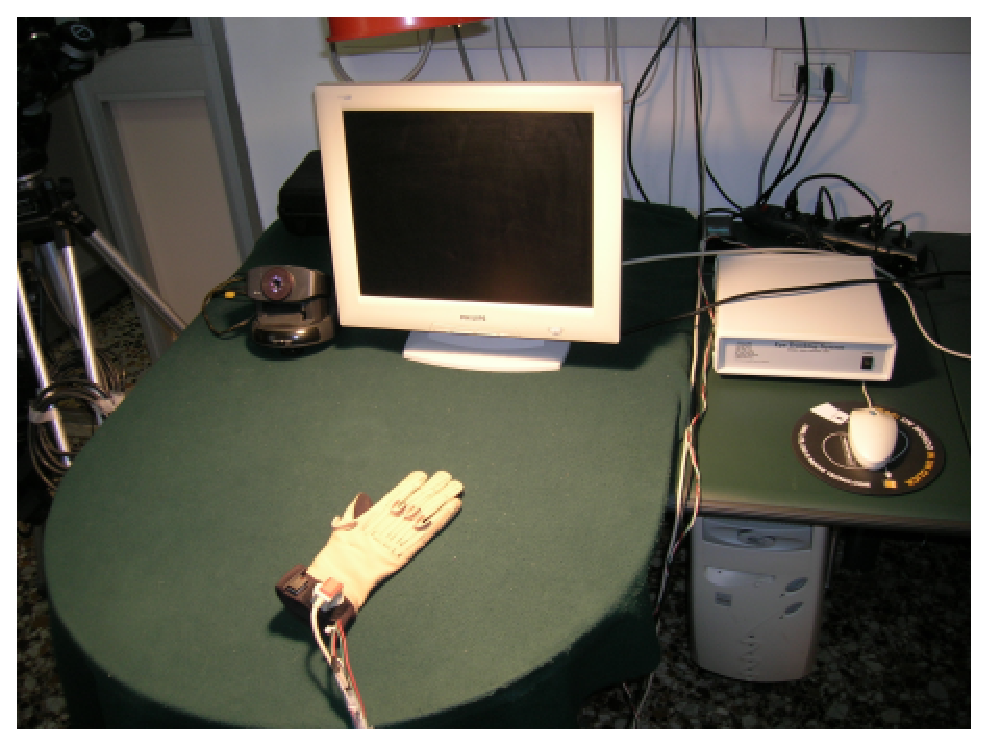
\includegraphics[width=0.31\linewidth]{setup.eps} \\
      $(a)$ & $(b)$ & $(c)$
    \end{tabular}
    \caption{The setup and devices used for the experiment: $(a)$ the
    Immersion CyberGlove with the Flock-of-Birds sensor just above the
    wrist; $(b)$ the ASL E504 gaze tracker (pan/tilt near-infrared
    camera); $(c)$ the whole setup.}
    \label{fig:devices}
\end{figure*}

Complex human/robotic interaction is a scenario in which a robotic
artifact must be timely and accurately guided by a human being, the
environmental conditions being hostile. A typical example is
teleoperation, consisting of having a robotic setup (the \emph{slave})
work in a remote environment, guided by a human user (the
\emph{master}). In a basic setting, the slave is reasonably humanoid
or at least intuitively controllable by the master; the master is
fully able-bodied; and the cooperation between master and slave is
realised in such a way that the actions performed by the master can be
precisely and timely replicated by the slave. In order to convey a
feeling of telepresence, in particular, a high bandwidth is required
for the slave-to-master sensorial feedback \cite{telesensation}.

But, when any of the above conditions fails, teleoperation must be
somehow augmented in order to keep on working. The slave could consist
of a set of surgical tools \cite{okamura} not immediately related to
the human fingers; or, the master could be a disabled person; or,
lastly, the master/slave communication bandwidth could be insufficient
for a timely and accurate transmission of sensorial feedback.

One of the possibilities to overcome these problems is that of making
the slave more intelligent by building into it \emph{internal models}
of the required actions \cite{kawato-99}. It is envisioned, in this
scenario, that the master should first train the slave to perform the
actions required, in a safe and controlled environment; and that this
acquired knowledge should then be used by the slave in real
situations, whenever the environment or the master's abilities do not
allow direct control. Upon detecting the master's intention to, e.g.,
grasp an object in its own workspace, the slave should take control
over, initiate and complete a grasping action possibly modelled upon
the user's style, and then return the control to the master. This is
what we call \emph{semi-autonomous teleoperation}.

As a minimum set of requirements, such a model should be

\begin{enumerate}

  \item \emph{Accurate.} It should be able to tell exactly when to
    start an autonomous grasp, avoiding doing it when not required
    (false positive).

  \item \emph{Light and fast} since it must be used in a real-time
    human-robot interaction scenario.

  \item \emph{Flexible.} It must adapt well to different subjects'
    parameters (speed of reach, direction of motion), abilities and
    intentions; and it must be trained in a reasonably short amount of
    time.

\end{enumerate}

The applications of such a general framework are huge, even outside
the domain of teleoperation; picture, for instance, a prosthetic hand
trained to grasp by an amputee's electromyographic signal, according
to the shape and affordances of the objects in the workspace; and
possibly, also trained to recognise the \emph{way} the subjects wants
to grasp a particular object. If the model works fine, the control by
the user could be greatly improved.

In this paper we investigate the possibility of building such an
internal model, employing a machine learning system based upon a
Support Vector Machine (SVM) \cite{BGV92}. In particular, we show the
results of an experiment in which seven subjects, of different ages
and with slightly different movement and gaze abilities, were placed
in a real teleoperation scenario; the subjects would then teach a SVM
to recognise when they wanted to grasp an object in the slave setup by
simply and naturally fixating the object, reaching for it and closing
their hand.

The outcome of the experiment is that such a model can actually be
built, and that it fulfills all the requirements enumerated above: it
is highly accurate; the solution achieved is extremely compact; and
these characteristics are largely independent of the subjects'
abilities. Lastly, the training phase is accomplished using about
$3.5$ minutes of data gathered in real-time from each subject, in the
worst case.

The paper is structured as follows: after a quick review of related
work, Section \ref{sec:mat} describes the materials and methods used
in the experiment; Section \ref{sec:res} shows the experimental
results, and Section \ref{sec:con} draws conclusions and outlines
future work.

\subsection*{Related work}

The work presented here can be seen as a simple instance of learning
by imitation. Training a machine learning system upon human movements
data essentially builds a model of the subject's motion parameters,
and this schema is common among animals and humans. Such models are
called \emph{internal models} (see, e.g.,
\cite{kawato-99,wolpert-03,mussaivaldi-00}); and there is now
evidence, represented by \emph{mirror neurons}
\cite{rizzolatti-04,gallese-96,rizzolatti-01}, that such models are a
somehow abstract representation of actions, since they are elicited
both when a subject performs an action, but also when it sees the same
action performed by a peer.

Building internal models of action through machine learning seems then
to be a promising idea. This has so far been primarily done via
signals obtained from more invasive devices than those we use; specific
cases are, e.g., \cite{black1} where cortical activity in monkeys is
used to reconstruct their movements, \cite{emg} where the
electromyographic signal is used, and \cite{yokoi} where f-MRI is
used, with an application to hand prosthetics \cite{yokoi2}.

%%%%%%%%%%%%%%%%%%%%%%%%%%%%%%%%%%%%%%%%%%%%%%%%%%%%%%%%%%%%%%%%%%%%%%%%%%%%%%%%
\section{MATERIALS AND METHODS}
\label{sec:mat}

In this Section we detail the process of gathering data from human
subjects and how we made them suitable for analysis by a machine
learning system.

\subsection{Subjects}

Seven subjects, four women and three men aged $30$ to $73$,
volunteered to join the experiment. They were all right-handed and
fully able-bodied, and were given no knowledge of the aim of the
experiment. Four of the subjects were slightly visually
impaired. Moreover, the wide variance in the age of the subjects gave
us a reasonable spectrum of velocities achieved when grasping objects.
This was supposed to increase the difficulty of the experiment,
especially as far as the gaze control is concerned, but at the same
time it should have given us a more realistic idea of how a learning
system could adapt to subjects with different motion/sight abilities.

\subsection{Setup and devices}

The subjects were asked to sit confortably in front of a clean
workspace, and a flat $17$ inches color monitor was placed in front of
them at a distance of about half a meter. They wore an Immersion
\emph{CyberGlove} data glove \cite{cyberglove} on their right hand,
and an Ascension \emph{Flock-of-Birds} (FoB) \cite{fob} magnetic
tracker was firmly mounted on top of their wrist. Lastly, an ASL
\emph{E504} gaze tracker \cite{e504} was placed on the left hand side
of the monitor. Figure \ref{fig:devices} shows the devices and setup.

The FoB returns six double-precision numbers describing the position
($x$, $y$ and $z$ in inches) and rotation (azimuth, elevation and roll
in degrees) of the sensor with respect to a magnetic basis mounted
about one meter away from the subject. Its resolution is $0.1$ inches
and $0.5$ degrees. The E504, after a careful calibration phase,
returns one true/false value, denoting validity of the gaze
coordinates, and two double-precision numbers indicating the
coordinates of the subject's gaze with respect to the monitor. The
CyberGlove was used as an on-off switch, to detect when the subject's
hand would close, by monitoring one of its sensors via a threshold.

The monitor showed the slave's workspace; the slave is the humanoid
platform Babybot \cite{babybotHum2005}. For the experiment we only
employed one of its colour cameras.

All data were collected, synchronised, and saved in real time at a
frequency of about $47$Hz.

\subsection{Method}

The subjects were asked to initially keep their right hand and arm in
a resting position. The monitor showed the slave's workspace, in which
several objects could be clearly seen, and a moving red cross
corresponding to the detected subject's gaze. The subjects were then
instructed, upon a request by the experimenter, to look at one of the
objects on the monitor and then to move their hand as if to reach and
grasp it, signalling the act of grasping by closing their right
hand. The red cross on the screen turned green when the hand was
closed, to confirm the grasping.

This fake grasping act was repeated for $15$ to $21$ times, each time
with a different object (therefore, toward a different position) seen
on the monitor. The maximum duration of the whole experiment for a
single subject was about $3.5$ minutes, resulting in no tiredness.

\subsection{Building the data set}
\label{subsec:dataset}

The first question was \emph{what} to monitor from the subjects'
data. A few intuitive considerations led us to consider $(a)$ the
average of the subjects' hand velocity, $(b)$ the variance of the
subjects' gaze coordinates and $(c)$ the information whether the
subjects' right hand was open or closed. Essentially, it is expected
that, when the user wants to grasp an object, he/she first
\emph{fixates} the desired object and then \emph{reaches} for it (see,
e.g., \cite{johansson01}); lastly, at some time after the beginning of
the reaching movement, he/she will close the right hand as if to
grasp, as instructed.

We then expect, while fixating, the gaze coordinates to hover around
the point on the screen where the desired object is seen, that is,
their standard deviation over some time to be \emph{small}; also we
expect, while reaching, the hand to move toward the object on the
screen, that is, the hand velocity components to be on average
\emph{large}. The instants in which the hand is closed will signal the
intention to grasp, whereas those when the hand is open will be taken
as negative examples. Data $(a)$ were easily obtained by
differentiating in time the hand position $x,y,z$ coordinates obtained
from the FoB, while $(b)$ and $(c)$ were obtained straight from the
E504 and the CyberGlove. (The samples corresponding to negative values
of the E504 validity flag were ignored, manually verifying that this
would not hamper the overall statistics.)

From each subject we obtained a sequence of $6$-tuples (the three hand
velocity coordinates, the two gaze coordinates and the open/closed
hand flag). The above considerations should be valid \emph{over a
certain time window}, characteristic of the fixation/reaching
operations --- call it $\tau$; and in general each subject will have a
different $\tau(i), i=1,\ldots,7$. Driven by this, we then decided to
feed the learning system the following data: for each user $i$ (and
therefore for each sequence) and for a range of different values $T_c$
attributed to $\tau(i)$, the \emph{hand velocity average values} over
$T_c$ (three real numbers) and the \emph{gaze position standard
deviations} over $T_c$ (two real numbers). Training was enforced by
requiring that the the system could guess, instant by instant, whether
the hand was closed or not. This was represented as an integer value,
in turn $1$ or $-1$. The problem of guessing when the subject wants to
grasp was thus turned into a typical supervised learning problem.

\subsection{Grasping speed}

In choosing the range for $T_c$, we were driven by the main
consideration that a moving time window should not be longer then the
interval of time between one grasping attempt and the following
one. In fact, a longer time window could trick the system into
considering data obtained during two or more independent grasping
attempts.

By examining all sequences we found out that the interval between one
grasping attempt and the following one lasted on average $7.1 \pm 1.8$
seconds. We then decided to let $T_c$ range in the interval
$0.1,\ldots,2$ seconds with a step of $0.05$ seconds, and then to also
check $T_c=3,4,5$ seconds.

In general, we expected to find a ``best'' value for $T_c$, which
would then be the required $\tau(i)$ for each user, figuring out that
shorter values would convey too little information about the ongoing
movement, and that longer ones would tend to incorporate too much
useless information about the resting periods of the subjects' hand
and gaze; we also expected the former effect to be more pronounced
than the latter one, since we had carefully chosen the maximum value
of $T_c$ in order for the time window not to cover more than one
grasping attempt on average.

\subsection{Support Vector Machines}
\label{subsec:svm}

Our machine learning system is based upon Support Vector Machines
(SVMs). Introduced in the early 90s by Boser, Guyon and Vapnik
\cite{BGV92}, SVMs are a class of kernel-based learning algorithms
deeply rooted in Statistical Learning Theory \cite{v-edbed-82}, now
extensively used in, e.g., speech recognition, object classification
and function approximation with good results \cite{Cristianini00}. For
an extensive introduction to the subject, see, e.g., \cite{Burges98}.

We are interested here in the problem of SVM classification, that is:
given a set of $l$ training samples $S=\{\xx_i,y_i\}_{i=1}^l$, with
$\xx_i \in \RR^m$ and $y_i \in \{-1,1\}$, find a function $f$, drawn
from a suitable functional space $\mathcal{F}$, which best
approximates the probability distribution of the source of the
elements of $S$. This function will be called a \emph{model} of the
unknown probability distribution. In order to decide whether a sample
belongs to either category, the sign of $f$ is considered, with the
convention that $sgn(f(\xx)) \geq 0$ indicates $y = 1$ and
vice-versa. In practice, $f(\xx)$ is a sum of $l$ elementary functions
$K(\xx,\yy)$, each one centered on a point in $S$, and weighted by
real coefficients $\alpha_i$:

\begin{equation} \label{eqn:sol}
  f(\xx) = \sum_{i=1}^l \alpha_i K(\xx,\xx_i) + b
\end{equation}

\noindent where $b \in \RR$. The choice of $K$, the so-called
\emph{kernel}, is done \emph{a priori} and defines $\mathcal{F}$ once
and for all; it is therefore crucial. According to a standard practice
(see, e.g., \cite{Cristianini00}) we have chosen a \emph{Gaussian}
kernel, which has one positive parameter $\sigma \in \RR$ which is the
standard deviation of the Gaussian functions used to build
(\ref{eqn:sol}). Notice that this is not related to the fact that the
target probability distribution might or might not be Gaussian.

Now, let $C \in \RR$ be a positive parameter; then the $\alpha_i$s and
$b$ are found by solving the following minimisation problem
(\emph{training phase}):

\begin{equation} \label{eqn:svm_primal}
  \arg \min_{\aa} \left( R(S,K,\aa) + C \sum_{i=1}^l L(\xx_i,y_i,f) \right)
\end{equation}

\noindent where $R$ is a \emph{regularisation term} and $L$ is a
\emph{loss functional}. In practice, after the training phase, some of
the $\alpha_i$s will be zero; the $\xx_i$s associated with non-zero
$\alpha_i$s are called \emph{support vectors}. Both the training time
(i.e., the time required by the training phase) and the testing time
(i.e., the time required to find the value of a point not in $S$)
crucially depend on the total number of support vectors; therefore,
this number is an indicator of how hard the problem is. Since the
number of support vectors is proportional to the sample set
\cite{Steinwart03}, an even better indicator of the hardness of the
problem is the percentage of support vectors with respect to the
sample set size. We will denote this percentage by the symbol $p_{SV}$
and call it \emph{size} of the related model. Willing to implement the
system on-line, one has to choose models with the smallest possible
size.

In (\ref{eqn:svm_primal}), minimising the sum of $R$ and $L$ together
ensures that the solution will approximate well the values in the
training set, at the same time avoiding overfitting, i.e., exhibiting
poor accuracy on points outside $S$. Smaller values of the parameter
$C$ give more importance to the regularisation term and vice-versa.

There are, therefore, two parameters to be tuned in our setting: $C$
and $\sigma$. In all our tests we found the optimal values of $C$ and
$\sigma$ by grid search with $3$-fold cross-validation. This ensures
that the obtained models will have a high generalisation power, i.e.,
their guess will be accurate also on samples not in $S$.

Notice, lastly, that the quantity to be minimised in Equation
(\ref{eqn:svm_primal}) is convex; due to this, as well as to the use
of a kernel, SVMs have the advantages that their training is
guaranteed to end up in a global solution and that they can easily
work in highly dimensional, non-linear feature spaces, as opposed to
analogous algorithms such as, e.g., artificial neural networks. As a
matter of fact, SVMs are best employed when the chosen kernel maps the
samples to a space in which the problem is \emph{linearly separable},
that is, a hyperplane (linear function) can be found which separates
the samples labelled $1$ from those labelled $-1$.

We have employed LIBSVM v2.82 \cite{ChangL01}, a standard, efficient
implementation of SVMs.

According to the procedure described in the previous parts of this
Section, we decided to set up a SVM for each user $i$ and value of the
time window $T_c$, defining $\RR^{5}$ as the input space: the hand
velocity average and gaze position standard deviation over
$T_c$. According to this, as is standard in SVM literature, the ranges
of the parameters $C$ and $\sigma$ were chosen as follows: $C$ was
$10^k$ with $k=-1,\ldots,3$, whereas $\sigma$ was
$\sqrt{\frac{5}{10^{k}}}$ with $k=-1,\ldots,3$.

%%%%%%%%%%%%%%%%%%%%%%%%%%%%%%%%%%%%%%%%%%%%%%%%%%%%%%%%%%%%%%%%%%%%%%%%%%%%%%%%
\section{EXPERIMENT RESULTS}
\label{sec:res}

This Section presents the results of our experiments, along with a
comparison with a simple baseline classification method which does not
employ SVMs. We here try to cover the issues raised in the
Introduction.

\subsection{Are SVMs really needed?}

One immediate consideration that comes to the experimenter's mind when
facing such a problem regards the difficulty of the problem. Since the
subjects kept their arm and hand still between grasping attempts, one
could think that a simple ``if/then/else'' method, based upon a
threshold for each coordinate of the input space, would suffice. As
noted above, the intuition is that, during the grasp (or maybe a
little sooner, depending on the value of $T_c$) the hand velocity
should be large while the gaze position standard deviation should be
small. Therefore, finding five thresholds and comparing instant by
instant the subjects' values with them could be enough. In other
words, SVMs could be not needed for solving the problem. \footnote{This
alternative approach is a simple instance of a \emph{decision
tree}. See, e.g., \cite{dtrees} for more details. A full comparison of
the two learning methods is out of the scope of this paper, but notice
that decision trees have been used, e.g., in fish motion recognition
\cite{fish}.}

In order to answer this question, at least partially, we ran our SVM
against such a simple threshold system. For each subject and for each
dimension of the input space (that is, for each hand velocity and gaze
position coordinate) we found out the maximum and minimum values over
the whole sequence, then subdivided this interval into $10$
parts. Lastly we exhaustively tried all $10^5$ possible thresholds
$(t_1,t_2,t_3,t_4,t_5)$ and picked up the choice which maximised the
accuracy. The thresholds were checked like this: if the values of the
hand velocity moving averages were larger than $(t_1,t_2,t_3)$ and the
values of the gaze position standard deviations were smaller than
$(t_4,t_5)$, then the system would guess the label $1$; it would guess
$-1$ otherwise. Indeed, if the accuracies achieved by the two systems
were comparable, one would be driven toward the simpler one, also
since, after having found the best thresholds, the testing time would
be constant and extremely small, making it ideal for real-time, online
processing.

Unfortunately, it turns out that such a simple threshold system won't
work well enough. Figure \ref{fig:comparison} shows the accuracy
achieved by the two systems.

\begin{figure}[htbp]
  \centering
    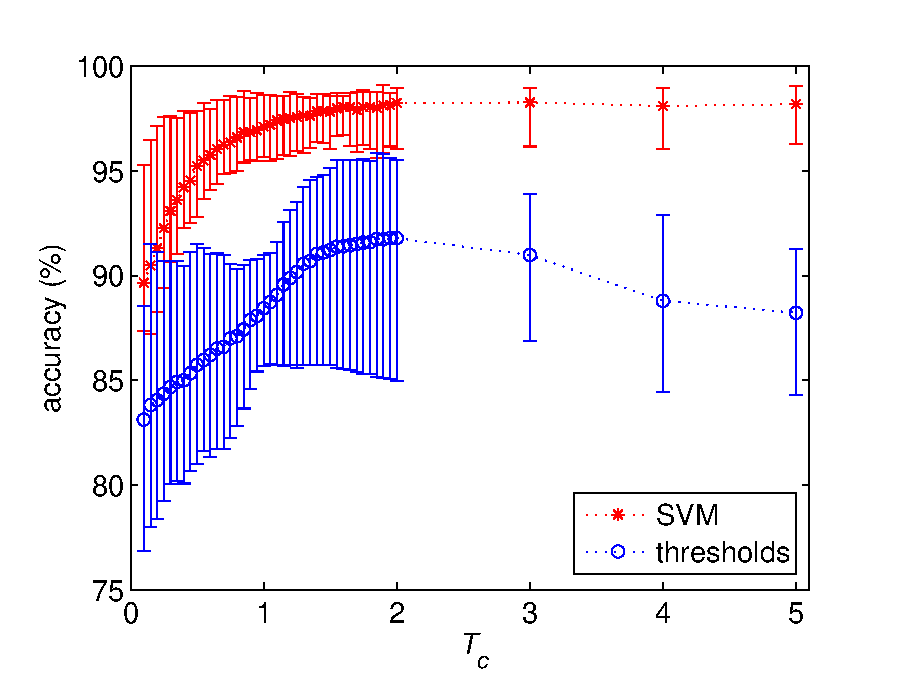
\includegraphics[width=\linewidth]{comparison.eps}
    \caption{Comparison between a simple threshold system and
    SVMs. The curves denote the average accuracy over all subjects,
    whereas the errorbars represent the minimum and maximum
    accuracies.}
    \label{fig:comparison}
\end{figure}

\begin{figure*}[!t]
  \centering
    \begin{tabular}{cc}
      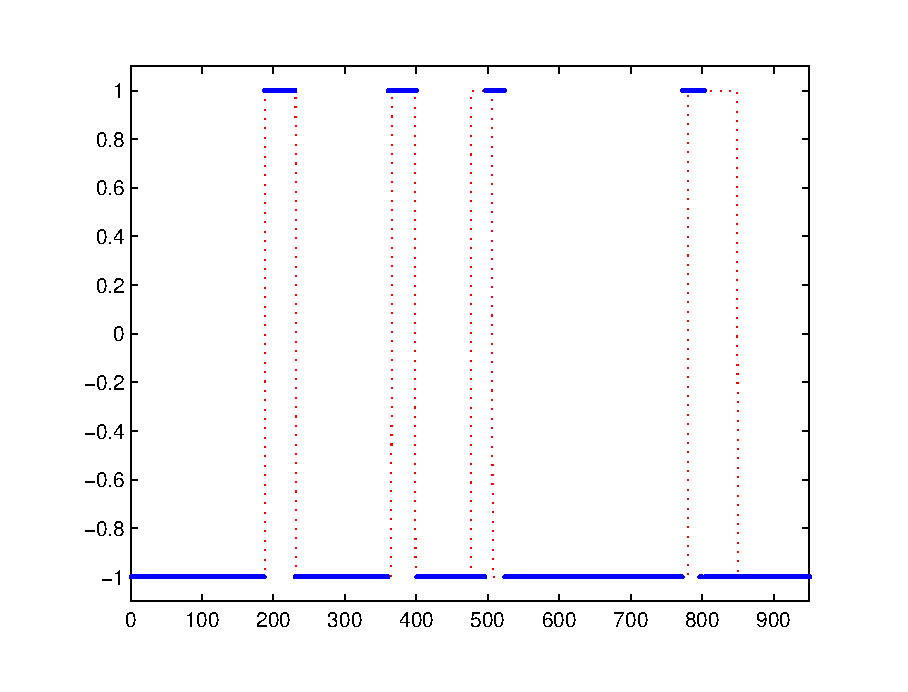
\includegraphics[width=0.45\textwidth]{predictionT.eps} &
      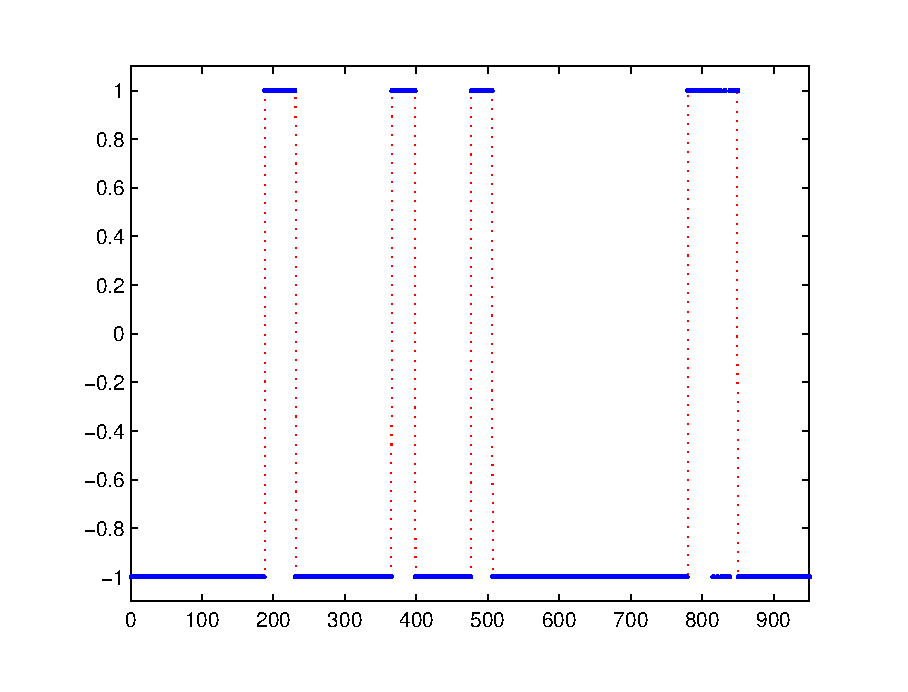
\includegraphics[width=0.45\textwidth]{predictionS.eps} \\
      $(a)$ & $(b)$
    \end{tabular}
    \caption{Predicted labels when $T_c=2$ for a particularly hard
    subject for SVMs (number $5$, a $73$-years old woman who has
    undergone a cataract operation). The graph shows $20$ seconds of
    data. $(a)$ Labels predicted by the threshold system. $(b)$
    Labels predicted by the SVM. The dotted red line indicates the
    true labels, whereas the blue spots are the predicted ones.}
    \label{fig:prediction}
\end{figure*}

The curves show the average accuracy over all the subjects, while the
error bars represent the minimum and maximum accuracies achieved by
each method. As one can see, SVMs are consistently and uniformly
better than the threshold system; moreover, there is basically no
overlapping between the error bars (except for a few points on the
left-hand side of the graph --- that is, where the accuracy is quite
low), indicating that there is almost no chance one can do better with
such a system than with SVMs, at least if one wishes to obtain a
reasonable accuracy. Notice, also, that the error bars are indeed
shorter in the case of SVMs, making it for a more robust (i.e., less
sensitive to the variance over the subjects) prediction.

A few more considerations will further justify the choice of a machine
learning schema. Firstly, there are strong hints that a threshold
system would not scale up to more complex and/or larger problems,
since the computational cost of such a method grows polynomially with
the number of subdivisions of each input space dimension, and
exponentially with the number of input space dimensions; moreover,
such a simple method is likely to be much more prone to noise
affecting the samples than SVMs are (picture a more realistic case in
which the subject, between grasping attempts, is doing ``something
else'' rather than keeping the arm still). In fact, employing such a
system is tantamount to defining the functional space of decision
surfaces $\mathcal{F}$ as the set of coordinate-wise half-spaces, as
opposed to the much richer space induced by a Gaussian kernel.

Secondly, it must be noted that the number of $1$ labels is much
smaller than that of $-1$ labels; actually, the average number of $1$s
is $17.1\% \pm 4.3\%$ of the whole set of labels. This is due to the
fact that the grasping act lasts a few tenths of a second and, for the
rest of the time, the subject is at rest.  As a consequence, a dumb
predictor which guessed $-1$ identically would achieve an average
accuracy of about $83\%$! When looking at accuracy values, it must
therefore be checked that the accuracy (percentage of correctly
predicted labels with respect to the total number of labels) is high
enough to ensure a sensible prediction, and it must be reminded that
an accuracy around $85\%$ is not much better than flipping a
coin.\footnote{A sensible alternative would be that of considering a
``weigthed'' accuracy $\frac{n_1 c_1 + n_{-1} c_{-1}}{c_1+c_{-1}}$,
where $n_i$ is the number of correctly guessed $i$ labels, $i \in
\{1,-1\}$ and $c_i$ is the total number of $i$ labels.} Considering
Figure \ref{fig:comparison} again in the light of this point, one
realises that the superior performance of SVMs is even more relevant:
at their best average accuracy (that is, for $T_c=2$), SVMs are
$96.04\%$ accurate whereas the threshold system gets a score of
$90.9\%$.

As a typical example, Figure \ref{fig:prediction} shows $20$ seconds
of predicted labels for $T_c=2$ for the most difficult subject for
SVMs, that is, subject $5$ (a 73-years old woman who has undergone in
the past a cataract surgical operation): as one can see, the threshold
system prediction shows a number of false positives and negatives,
whereas the SVM prediction suffers of only a few false negatives.

\subsection{Accuracy}
\label{subsec:accuracy}

\begin{figure*}[!t]
  \centering
    \begin{tabular}{cc}
      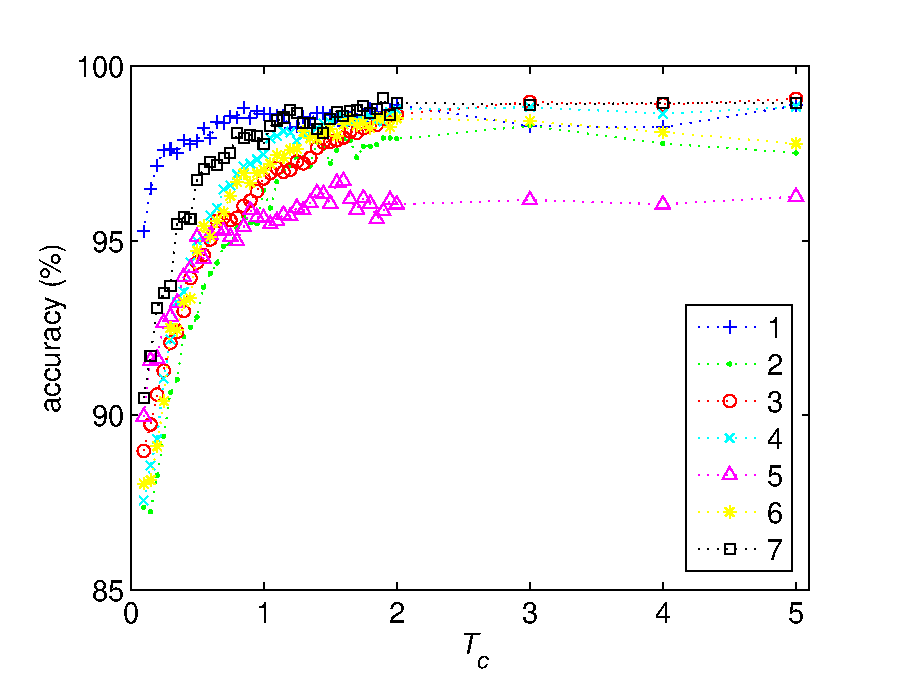
\includegraphics[width=0.45\textwidth]{accuracy.eps} &
      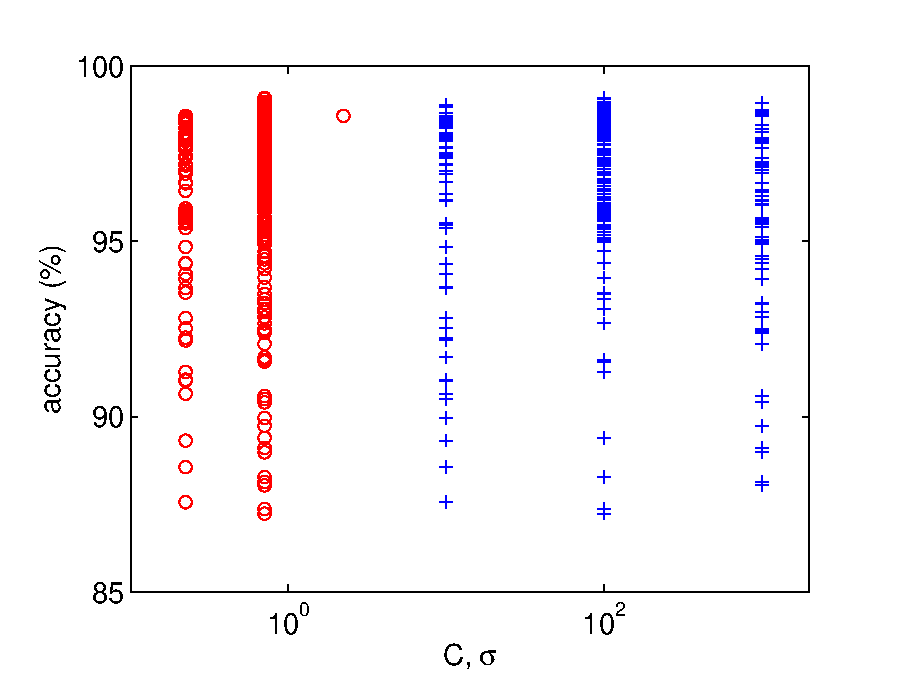
\includegraphics[width=0.45\textwidth]{hyperparams.eps} \\
      $(a)$ & $(b)$
    \end{tabular}
    \caption{Accuracy obtained by the SVM and related values of the
    parameters $C$ and $\sigma$ found by grid search. $(a)$ Accuracy
    curve for each subject (numbered $1$ to $7$), as the time window
    $T_c$ varies; $(b)$ the values of $C$ (blue ``plus'' symbols) and
    $\sigma$ (red circles) versus the accuracy.}
    \label{fig:accuracy}
\end{figure*}

\begin{figure*}[!t]
  \centering
    \begin{tabular}{cc}
      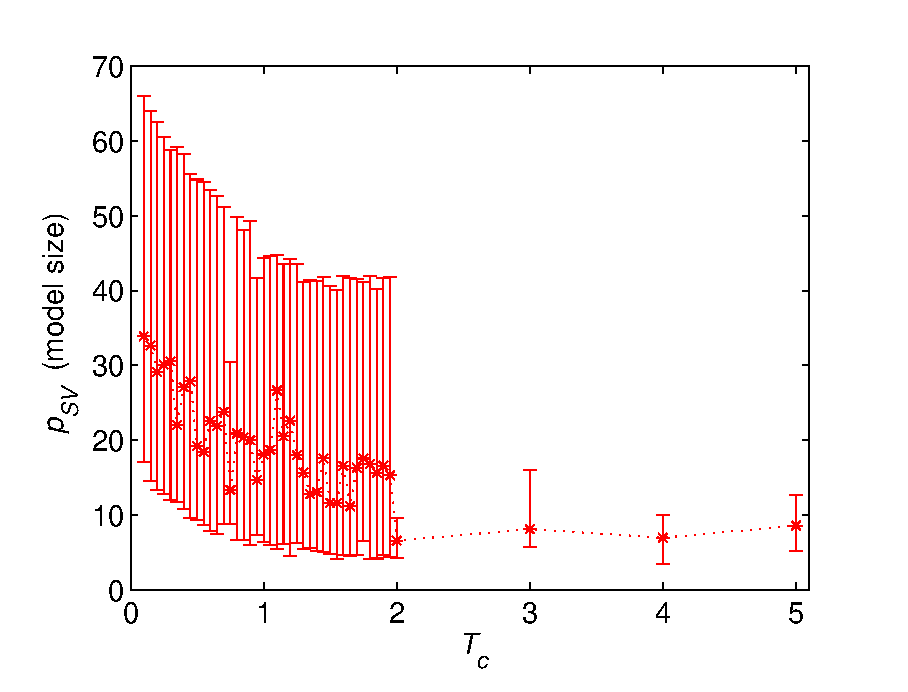
\includegraphics[width=0.45\linewidth]{SVs.eps} &
      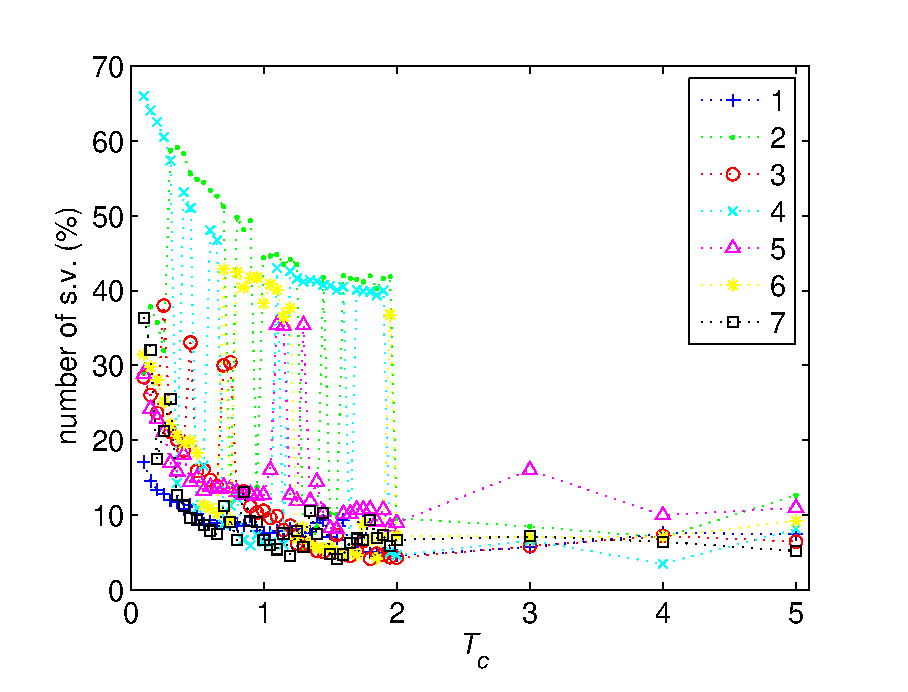
\includegraphics[width=0.45\textwidth]{svs_subj.eps} \\
      $(a)$ & $(b)$
    \end{tabular}
    \caption{Model size as $T_c$ grows. $(a)$ The points denote the
    average size over all subjects, whereas the error bars represent
    the minimum and maximum size. $(b)$ The same graph, but one curve
    for each subject.}
    \label{fig:svs}
\end{figure*}

Figure \ref{fig:accuracy} $(a)$ shows the accuracy attained by the SVM
for each subject separately, numbered $1$ to $7$; Figure
\ref{fig:accuracy} $(b)$ shows the values of $C$ and $\sigma$ versus
the accuracy, obtained by grid search as detailed in the previous
Section. Figure \ref{fig:accuracy} $(a)$ is essentially a more
detailed version of the red curve in Figure \ref{fig:comparison}.

Consider Figure \ref{fig:accuracy} $(a)$: it is apparent that SVMs
attain an excellent result on all subjects. The maximum accuracy is
attained, depending on the subject, for $T_c$ between $1.5$ and $2$
seconds, and ranges from about $99\%$ (subjects $3$ and $7$) to
$96.71\%$ (subject $5$, not surprisingly). All curves seem to reach
the maximum accuracy as $T_c$ grows, and then keep roughly
constant. This is somehow surprising, also taking into account that,
for the threshold system (recall Figure \ref{fig:comparison}, blue
curve), the accuracy degrades as a longer and longer time window is
considered.

As far as the subjects' abilities are concerned, the only obviously
worse result is obtained on subject $5$, who is supposed to have a
rather different kinematic behaviour than the others, because of her
age, and poses severe problems to the gaze tracker calibration since
her eyes have been surgically operated. Subject $2$, also showing a
slightly worse performance than the others, suffers of a rare form of
eye disease. All in all, however, it seems that visual impairments do
not significantly hinder the accuracy attained by the SVM.

An interesting point for this analysis, moreover, comes from the
observation of the distribution of the parameters' values versus the
accuracy (Figure \ref{fig:accuracy} $(b)$). First of all, notice that
$C$ only takes values $10$, $100$ and $1000$, and that $\sigma$, with
just one exception, only takes values $0.2236$ and $0.7071$ (that is,
recall Subsection \ref{subsec:svm}, $\sqrt{\frac{5}{10^{k}}}$ with
$k=1,2$). Checking which ``stripes'' are more dense where the accuracy
is higher, we find that good values for the parameters are $C=100$ and
$\sigma=0.7071$. These values, taking into account that the input
space has dimension $5$, are pretty standard values denoting a rather
easy problem; in particular, a value of $100$ for $C$ denotes that, in
Equation \ref{eqn:svm_primal}, the regularisation term has little
importance, or, which is equivalent, that the problem is well linearly
separated in the feature space. This is one more point in favour of
the specific use of a Gaussian kernel SVM approach for this
problem.

\subsection{Size of the models}

Again, recall Subsection \ref{subsec:svm}. We checked the model size
for each value of $T_c$: the smaller the size, the better. Figure
\ref{fig:svs} $(a)$ plots the size of each model as $T_c$ grows. The
curve shows the average size over all subjects, while the error bars
represent the minimum and maximum size.

Interestingly, as $T_c$ grows (and therefore as the accuracy grows,
recall Figure \ref{fig:comparison}, red plot), the size of the related
model \emph{decreases}. This in general indicates that the problem is
more and more tractable, as fewer and fewer support vectors are
required to faithfully represent the decision surface. Notice,
however, that the error bars are rather wide up to $T_c=2$, the
support vectors being anyway as many as $40\%$ of the total samples in
the best case ($T_c=1.85$, average $15.64\%$, minimum $4.16\%$,
maximum $40.26\%$. It is not clear why the error bars drop so sharply
for $T_c=2,3,4,5$ --- a finer analysis of the behaviour of the models
size is required for $T_c>2$).

It would then seem that there is little chance to obtain a model which
is \emph{both accurate and small} for all subjects, uniformly; but a
deeper analysis of these data reveals an interesting
phenomenon. Figure \ref{fig:svs} $(b)$ shows the actual model sizes
subject by subject. It is from this Figure apparent that the size
presents wide oscillations corresponding to small changes in $T_c$,
while maintaining a decreasing trend. As an example, subject $2$ has
$p_{SV}=43.49\%$ when $T_c=1.25$ seconds, but drops to $p_{SV}=5.48\%$
when $T_c=1.3$ seconds!

The reason of these oscillations is that parameter grid search is done
by taking the parameter values corresponding to the model with best
accuracy, regardless of the size. Small changes in the accuracy can
then drive the search toward much bigger or smaller models. This
phenomenon enables us to find at least one distinct (possibly best)
value of $T_c$ for each subject, such that in that point the
corresponding model is both accurate and small.

\begin{figure*}[!t]
  \centering
    \begin{tabular}{cc}
      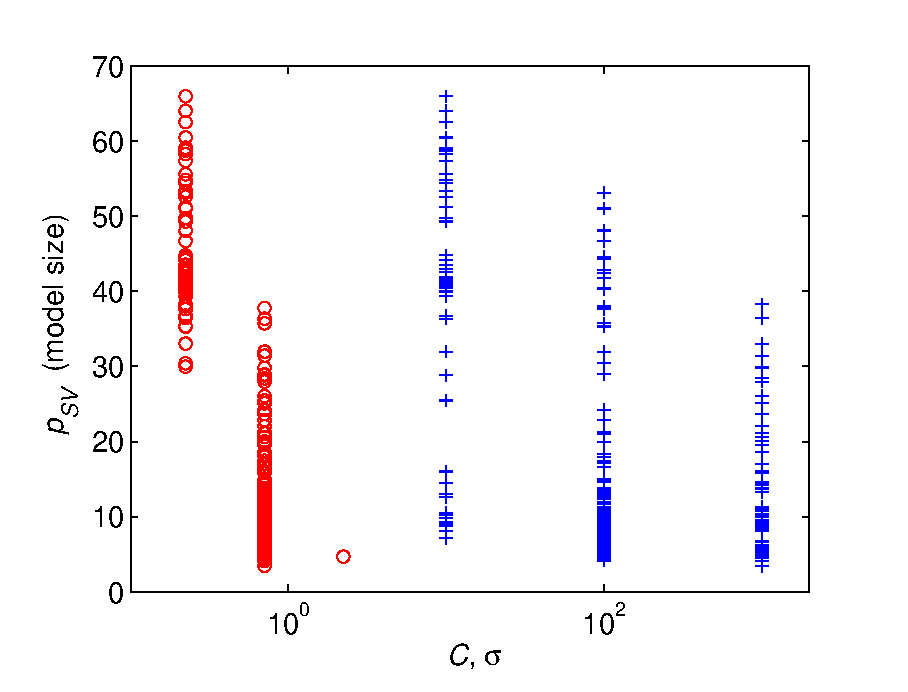
\includegraphics[width=0.45\textwidth]{svs_params.eps} &
      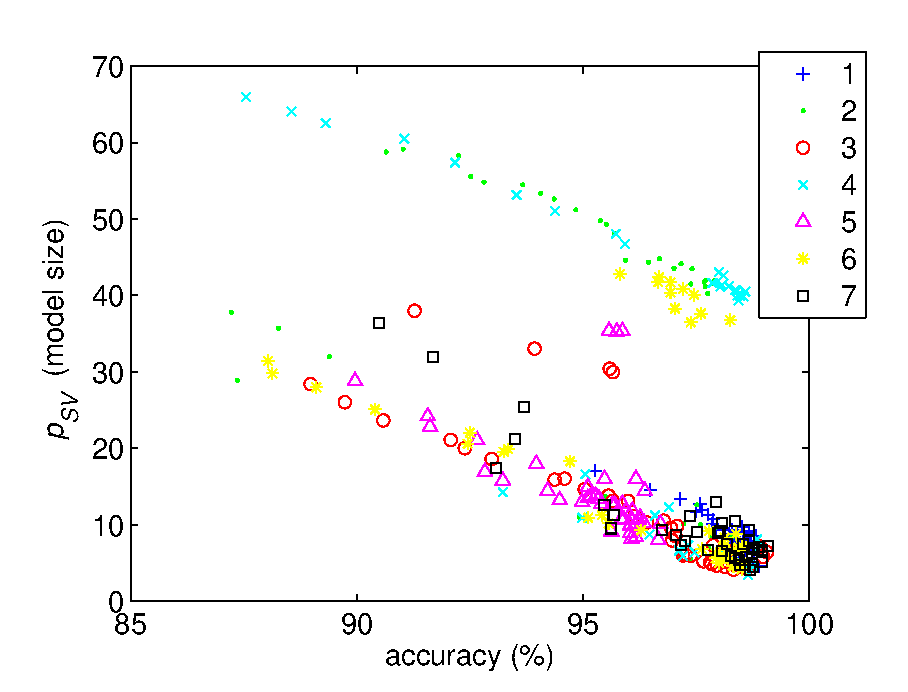
\includegraphics[width=0.45\textwidth]{acc_svs.eps} \\
      $(a)$ & $(b)$
    \end{tabular}
    \caption{$(a)$ Model size versus the parameters $C$ (blue ``plus''
    symbols) and $\sigma$ (red circles). While $C$ seems largely
    ininfluent on the size, with a certain preference for $C=100$, for
    $\sigma=0.7071$ the models are much smaller, getting a $p_{SV}$ as
    small as $3.45\%$. $(b)$ For each model, coloured according to the
    subject it belongs to, size versus accuracy. The models are
    grouped into two clusters, one of accurate but large models (upper
    right corner) and one of accurate and small models (lower right
    corner). Both clusters display a precise trend: the higher the
    accuracy, the smaller the models.}
    \label{fig:svs_params}
\end{figure*}

Consider Figure \ref{fig:svs_params} $(a)$, plotting the parameters
$C$ and $\sigma$ like in Figure \ref{fig:accuracy} $(b)$, but this
time versus the size: it turns out that the smallest models have
$C=100$, but this is a vague indication, since other values of $C$
attain small models, too; but that $\sigma=0.7071$ is definitely the
best value, since when $\sigma=0.2236$ the models are indeed
larger. Interestingly, these good values match those found in
Subsection \ref{subsec:accuracy}.

We still have to check that these values are not tuned upon a certain
(subset of) subject(s); if that were the case, there would still be
some subjects for which no accurate and small models could be
found. As it turns out, this is not the case: by looking at Figure
\ref{fig:svs_params} $(b)$, one realises that there are indeed
accurate and small models for every subject (the points in the lower
right corner cluster). The two clusters correspond to the wide
oscillations in size observed in Figure \ref{fig:svs} $(b)$. It turns
out that the upper right corner cluster in Figure \ref{fig:svs_params}
$(b)$ is characterised by $\sigma=0.2236$, whereas the lower right
corner cluster has $\sigma=0.7071$. The Figure also tells us that
there is a trend in both clusters, associating accuracy and small
size.

\subsection{Flexibility}

Lastly: can we then say that SVMs produce ``good'' models for each
subject? Based upon the considerations in the previous Subsection, we
can define, for each subject, a notion of ``best'' model as the one
which is lowest and rightmost in \ref{fig:svs_params} $(b)$, that is,
which is the most accurate and smallest for that subject. To each of
these models, and therefore to each subject, a values of $T_c$ is
associated, and this will be the $\tau(i)$ mentioned in the Subsection
\ref{subsec:dataset}. Table \ref{tab:tau} lists the models found,
along with their characteristics, for each subject.

\begin{table}[!t]
  \centering
    \caption{Best model found for each subject.}
    \begin{tabular}{|r|r|r|r|}
      \hline
      Subj. & Acc. & $p_{SV}$ & $\tau(i)$ \\
      \hline
      1 & 98.90\% & 4.56\% & 2   \\
      2 & 97.38\% & 5.48\% & 1.3 \\
      3 & 98.32\% & 4.14\% & 1.8 \\
      4 & 98.64\% & 3.45\% & 4   \\
      5 & 96.66\% & 8.08\% & 1.55\\
      6 & 98.50\% & 4.16\% & 1.85\\
      7 & 98.70\% & 4.13\% & 1.55\\
      \hline
    \end{tabular}
    \label{tab:tau}
\end{table}

As expected, there is a model for each user which is both accurate
(ranging from $98.9\%$ to $96.66\%$ accuracy) and small (ranging from
$p_{SV}=3.45\%$ to $p_{SV}=8.08\%$). Consistently, the worst model is
that of subject $5$. All models have $C=100$ or $C=1000$ and
$\sigma=0.7071$, as predicted. The characteristic time windows
$\tau(i)$ range from $1.3$ seconds to $4$ seconds (in this latter
case, again, a finer analysis of large values of $T_c$ is required).

%%%%%%%%%%%%%%%%%%%%%%%%%%%%%%%%%%%%%%%%%%%%%%%%%%%%%%%%%%%%%%%%%%%%%%%%%%%%%%%%
\section{CONCLUSIONS AND FUTURE WORK}
\label{sec:con}

In this paper we have tried to obtain good artificial internal models
of when to grasp by applying Support Vector Machines to data gathered
from diverse human subjects, engaged in a simple grasping experiment in
a teleoperation scenario.

The experimental results and related analysis reveals that the
approach is definitely successful. First of all, the problem is not
trivial and cannot be efficiently solved by means of a na\"\i ve
approach such as a cascade of if/then/else rules; it is, on the other
hand, solved very well by a SVM with Gaussian kernel, and there are
hints that this approach is particularly well suited for the problem,
since the analysis of the paramters obtained for the best models on
each subject reveals a good degree of linear separation of the data
\emph{in the feature space}.

The models obtained for each subject are $(a)$ highly accurate, giving
the correct guess in $98.9\%$ to $96.66\%$ of the cases; $(b)$ small,
and therefore fast and usable in an on-line environment, the
percentage of support vectors for each model ranging from $3.45\%$ to
$8.08\%$ of the sample set; and $(c)$ flexible, able to find an
optimal characteristic time window for each subject, in the range from
$1.3$ seconds to $4$ seconds.

Future work is open and stimulating. As far as SVMs are concerned, a
deeper analysis of the behaviour of SVMs when $T_c>2$ is required, as
well as a finer and smarter way of doing grid search for the SVM
paramters. From a more abstract and general point of view, one might
wonder what the deep meaning is of the few support vectors collected
for each subject in the best models: are there any similarities among
them across the subjects? In other words, do they represent common
characteristics of the human act of grasping? If so, their accuracy
should be transferrable across subjects.

Lastly, are the common characteristics of the best models somehow
related to the kinematics of human reaching and fixating? And, can
they effectively be trasferred to more complex, real-life scenarios
such as, e.g., semi-autonomous teleoperation in a hostile environment,
or with a disabled master? Can they be used to build semi-autonomous
prostheses? These questions will be answered in future research.

%%%%%%%%%%%%%%%%%%%%%%%%%%%%%%%%%%%%%%%%%%%%%%%%%%%%%%%%%%%%%%%%%%%%%%%%%%%%%%%%
\section*{ACKNOWLEDGMENTS}

The work is supported by the EC project NEURObotics
(FP6-IST-001917). We thank Giorgio Metta of the Italian Institute of
Technology and Francesco Orabona of the LIRA-Lab for their support.

%%%%%%%%%%%%%%%%%%%%%%%%%%%%%%%%%%%%%%%%%%%%%%%%%%%%%%%%%%%%%%%%%%%%%%%%%%%%%%%%

\IEEEtriggeratref{12}

{\small
\bibliographystyle{unsrt}
\bibliography{paper}
}

\end{document}
